% Copyright © 2012 Martin Ueding <dev@martin-ueding.de>
%
\documentclass[11pt, ngerman, fleqn]{article}

\usepackage[a4paper, left=3cm, right=2cm, top=2cm, bottom=2cm]{geometry}
\usepackage[activate]{pdfcprot}
\usepackage[cdot, squaren]{SIunits}
\usepackage[iso]{isodate}
\usepackage[parfill]{parskip}
\usepackage[T1]{fontenc}
\usepackage[utf8]{inputenc}
\usepackage{amsmath}
\usepackage{amsthm}
\usepackage{babel}
\usepackage{color}
\usepackage{commath}
\usepackage{epstopdf}
\usepackage{fancyhdr}
\usepackage{graphicx}
\usepackage{hyperref}
\usepackage{lastpage}
\usepackage{setspace}
\usepackage{tikz}

\usepackage[charter, greekuppercase=italicized]{mathdesign}

\definecolor{darkblue}{rgb}{0,0,.5}
\definecolor{darkgreen}{rgb}{0,.5,0}

\hypersetup{
	breaklinks=false,
	citecolor=darkgreen,
	colorlinks=true,
	linkcolor=black,
	menucolor=black,
	urlcolor=darkblue,
}

\setlength{\columnsep}{2cm}

\DeclareMathOperator{\arcsinh}{arsinh}
\DeclareMathOperator{\arsinh}{arsinh}
\DeclareMathOperator{\asinh}{arsinh}
\DeclareMathOperator{\card}{card}
\DeclareMathOperator{\diam}{diam}

\newcommand{\dalambert}{\mathop{{}\Box}\nolimits}
\newcommand{\divergence}[1]{\inner{\vnabla}{#1}}
\newcommand{\ee}{\mathrm e}
\newcommand{\emesswert}{\del{\messwert \pm \messwert}}
\newcommand{\e}[1]{\cdot 10^{#1}}
\newcommand{\fehlt}{\textcolor{red}{Hier fehlen noch Inhalte.}}
\newcommand{\half}{\frac 12}
\newcommand{\ii}{\mathrm i}
\newcommand{\inner}[2]{\left\langle #1, #2 \right\rangle}
\newcommand{\laplace}{\mathop{{}\Deltaup}\nolimits}
\newcommand{\messwert}{\textcolor{blue}{\square}}
\newcommand{\punkte}{\textcolor{white}{xxxxx}}
\newcommand{\tens}[1]{\boldsymbol{#1}}
\newcommand{\vnabla}{\vec \nabla}
\renewcommand{\vec}[1]{\boldsymbol{#1}}

\newcommand{\themodul}{math340}
\newcommand{\thegruppe}{Gruppe 16 -- Malte Lackmann}
\newcommand{\theuebung}{5}

\pagestyle{fancy}

\fancyfoot[C]{\footnotesize{\thegruppe}}
\fancyfoot[L]{\footnotesize{Ueding, Manz, Lemmer}}
\fancyfoot[R]{\footnotesize{Seite \thepage\ / \pageref{LastPage}}}
\fancyhead[L]{\themodul{} -- Übung \theuebung}

\def\thesection{\theuebung.\arabic{section}}
\def\thesubsection{\thesection\alph{subsection}}

\title{\themodul{} -- Übung \theuebung \\ \vspace{0.5cm} \large{\thegruppe}}

\author{
	Martin Ueding \\ \small{\href{mailto:mu@uni-bonn.de}{mu@uni-bonn.de}}
	\and
	Paul Manz
	\and
	Lino Lemmer
}

\begin{document}

\maketitle

\begin{table}[h]
	\centering
	\begin{tabular}{l|c|c|c|c}
		Aufgabe & \ref{1} & 5.3 & \ref{3} & $\sum$   \\
		\hline
		Punkte & \punkte / 4 & \punkte / 5 & \punkte / 6 & \punkte / 15
	\end{tabular}
\end{table}

%%%%%%%%%%%%%%%%%%%%%%%%%%%%%%%%%%%%%%%%%%%%%%%%%%%%%%%%%%%%%%%%%%%%%%%%%%%%%%%
%             Anfangswertaufgabe für die Wärmeleitungsgleichung             %
%%%%%%%%%%%%%%%%%%%%%%%%%%%%%%%%%%%%%%%%%%%%%%%%%%%%%%%%%%%%%%%%%%%%%%%%%%%%%%%

\section{Anfangswertaufgabe}
\label{1}

In die Lösungsformel eingesetzt erhalten wir:
\[
	u(x,t) = \frac{1}{\sqrt{4\pi t}} \int_{-\infty}^\infty \dif y \exp\del{
		- \frac{(x-y)^2}{4t} - y^2
	}
\]


Ich führe $\xi$ als neue Koordinate ein \cite{math.se-heat}:
\[
	\xi := \sqrt{\frac{1+4t}{4t}} \del{y-\frac{x}{1+4t}}
\]

Nun können wir das negative Argument der Exponentialfunktion umschreiben:
\begin{align*}
	\frac{(x-y)^2}{4t} + y ^2
	&= \frac{(1+4t) y^2 - 2xy + x^2}{4t} \\
	&= \frac{1+4t}{4t} \del{y^2-\frac{2x}{1+4t}y+\frac{x^2}{1+4t}} \\
	&= \frac{1+4t}{4t} \del{\del{y-\frac{x}{1+4t}}^2+\frac{x^2}{1+4t}-\frac{x^2}{(1+4t)^2}} \\
	&= \frac{1+4t}{4t} \del{\del{y-\frac{x}{1+4t}}^2+\frac{4x^2t}{(1+4t)^2}} \\
	&= \frac{1+4t}{4t} \del{y-\frac{x}{1+4t}}^2 + \frac{x^2}{1+4t} \\
	&= \xi^2 + \frac{x^2}{1+4t}
\end{align*}

Dies können wir nun in die Lösungsformel einsetzen und erhalten mit
$\dif y = \sqrt{\frac{4t}{1+4t}} \dif \xi$ und $\xi(\pm \infty) = \pm \infty$:
\begin{align*}
	u(x,t)
	&= \frac{1}{\sqrt{4\pi t}} \int_{-\infty}^\infty \dif y \exp\del{
		- \frac{(x-y)^2}{4t} - y^2
	} \\
	&= \frac{1}{\sqrt{4\pi t}} \sqrt{\frac{4t}{1+4t}} \int_{-\infty}^\infty \dif \xi \exp\del{
		- \del{\xi^2 + \frac{x^2}{1+4t}}
	} \\
	&= \frac{1}{\sqrt{\pi (1+4t)}} \exp\del{ - \frac{x^2}{1+4t} }
	\int_{-\infty}^\infty \dif \xi
	\exp\del{
		- \xi^2
	} \\
	\intertext{Das Integral ist einfach nur $\sqrt{\pi}$, dies kann man durch Quadrieren und Wechsel in Polarkoordinaten bestimmen.}
	&= \frac{1}{\sqrt{1+4t}} \exp\del{ - \frac{x^2}{1+4t} }
\end{align*}

Für $t = 0$ kommt gerade $\ee^{-x^2}$ heraus, wie gefordert. Die Funktion ist
in Abbildung \ref{fig:1-plot} gezeigt.

\begin{figure}
	\centering
	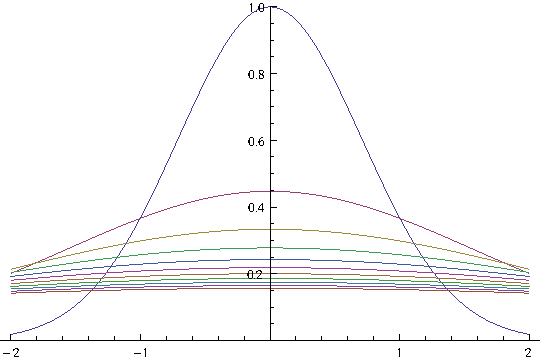
\includegraphics[width=0.5\textwidth]{1-plot.pdf}
	\caption{Plot von $u(x, t)$ für $t = 0, \ldots, 10$. Der höhste Graph ist $t=0$.}
	\label{fig:1-plot}
\end{figure}

\stepcounter{section}
\stepcounter{section}

%%%%%%%%%%%%%%%%%%%%%%%%%%%%%%%%%%%%%%%%%%%%%%%%%%%%%%%%%%%%%%%%%%%%%%%%%%%%%%%
%                               $g$ fortsetzen                                %
%%%%%%%%%%%%%%%%%%%%%%%%%%%%%%%%%%%%%%%%%%%%%%%%%%%%%%%%%%%%%%%%%%%%%%%%%%%%%%%

\section{$g$ fortsetzen}
\label{3}

Wir schreiben $\dot u := \pd ut$ und $u'' := \pd[2] ux$.

\subsection{homogen, Dirichlet}
\label{a}

Gegeben ist $\dot u = u''$ und $u(0, t) = 0$ sowie $u(x, 0) = g(x)$.

Im Nullpunkt muss $u=0$ gelten. Also setzen wir $g$ ungerade fort:
\[
	\tilde g(x) := \begin{cases}
		g(x) & x \geq 0 \\
	  -g(-x) & x < 0
	\end{cases}
\]

Dies setzen wir in die Lösungsformel ein:
\begin{align*}
	u(x, t)
	&= \frac{1}{\sqrt{4\pi t}} \int_{-\infty}^{\infty} \dif y \exp\del{- \frac{(x-y)^2}{4t}} \tilde g(y) \\
	&= \frac{1}{\sqrt{4\pi t}} \del{
		- \int_{-\infty}^{0} \dif y \exp\del{- \frac{(x-y)^2}{4t}} g(-y)
		+ \int_{0}^{\infty} \dif y \exp\del{- \frac{(x-y)^2}{4t}} g(y)
	} \\
	\intertext{Mit $z := -y$ und $\dif z = - \dif y$:}
	&= \frac{1}{\sqrt{4\pi t}} \del{
		\int_{\infty}^{0} \dif z \exp\del{- \frac{(x+z)^2}{4t}} g(z)
		+ \int_{0}^{\infty} \dif y \exp\del{- \frac{(x-y)^2}{4t}} g(y)
	} \\
	\intertext{Wir kehren die Integralgrenzen um und fassen die Integrale zusammen.}
	&= \frac{1}{\sqrt{4\pi t}}
		\int_{0}^{\infty} \dif y \del{ - \exp\del{- \frac{(x+y)^2}{4t}}
	+ \exp\del{- \frac{(x-y)^2}{4t}} } g(y)
	\\
	&= \frac{1}{\sqrt{4\pi t}}
		\int_{0}^{\infty} \dif y \exp\del{- \frac{x^2+y^2}{4t}}
	\del{- \exp\del{- \frac{2xy}{4t}} + \exp\del{\frac{2xy}{4t}} } g(y)
	\\
	\intertext{Dies ist gerade der doppelte $\sinh$.}
	&= \frac{1}{\sqrt{\pi t}}
		\int_{0}^{\infty} \dif y \exp\del{- \frac{x^2+y^2}{4t}}
	\sinh\del{\frac{2xy}{4t}} g(y)
\end{align*}

\subsection{homogen, Neumann}

Diese Aufgabe ist ähnlich Aufgabe \ref a, allerdings soll hier nicht $u(0, t) = 0$, sondern $u'(0, t) = 0$ gelten. Die Funktion $g$ setzen wir daher gerade fort, damit die Steigung immer $0$ bleibt:
\[
	\tilde g(x) := \begin{cases}
		g(x) & x \geq 0 \\
	  g(-x) & x < 0
	\end{cases}
\]

Dies setzen wir auch in die Lösungsformel ein. Der einzige Unterschied zur \ref 1 ist, dass ein Minuszeichen fehlt. Somit kommt nicht $\sinh$ sondern $\cosh$ am Ende heraus:
\[
	u(x, t) = \frac{1}{\sqrt{\pi t}}
		\int_{0}^{\infty} \dif y \exp\del{- \frac{x^2+y^2}{4t}}
	\cosh\del{\frac{2xy}{4t}} g(y)
\]

\subsection{inhomogen, Dirichlet}

Gegeben ist $\dot u = u'' - u$ und $u(0, t) = 0$ sowie $u(x, 0) = g(x)$. Als
Ansatz soll $u(x, t) = \ee^{-t} v(x, t)$ benutzt werden.

Die Ableitungen von $u$ sind:
\[
	u'' = \ee^{-t} v''
	,\quad
	\dot u = - \ee^{-t} v + \ee^{-t} \dot v
\]

Dies setzen wir in die Differentialgleichung ein und erhalten:
\[
	- \ee^{-t} v + \ee^{-t} \dot v = \ee^{-t} v'' - \ee^{-t} v
\]

Daraus folgt:
\[
	\dot v = v''
\]

Somit muss $v$ die normale Wärmeleitungsgleichung erfüllen. Außerdem soll $u(0,
t) = 0$ erfüllt sein. Die ist äquivalent zu $v(0, t) = 0$. Aus $u(x, 0) = g(x)$
können wir $v(x, 0) = g(x)$ folgern. Somit haben wir das Problem auf die
Aufgabe \ref a zurückgeführt. Das $u$ was wir dort erhalten haben, ist hier das
$v$. Zusammen mit $\ee^{-t}$ ergibt es die Lösung $u$.
\[
	u(x, t) = \frac{1}{\sqrt{\pi t}}
	\ee^{-t} \int_{0}^{\infty} \dif y \exp\del{- \frac{x^2+y^2}{4t}}
	\sinh\del{\frac{2xy}{4t}} g(y)
\]

\bibliography{../../zentrale_BibTeX/Central}
\bibliographystyle{plain}

\end{document}

.. vim: spell spelllang=de
